\documentclass[a4paper,12pt]{article}

%%% Работа с русским языком
\usepackage{cmap}					% поиск в PDF
\usepackage{mathtext} 				% русские буквы в формулах
\usepackage[T2A]{fontenc}			% кодировка
\usepackage[utf8]{inputenc}			% кодировка исходного текста
\usepackage[english,russian]{babel}	% локализация и переносы
\usepackage{xcolor}
\usepackage{hyperref}
 % Цвета для гиперссылок
\definecolor{linkcolor}{HTML}{00FFFF} % цвет ссылок
\definecolor{urlcolor}{HTML}{4682B4} % цвет гиперссылок

\hypersetup{pdfstartview=FitH,  linkcolor=linkcolor,urlcolor=urlcolor, colorlinks=true}

%%% Дополнительная работа с математикой
\usepackage{amsfonts,amssymb,amsthm,mathtools} % AMS
\usepackage{amsmath}
\usepackage{icomma} % "Умная" запятая: $0,2$ --- число, $0, 2$ --- перечисление

%% Номера формул
%\mathtoolsset{showonlyrefs=true} % Показывать номера только у тех формул, на которые есть \eqref{} в тексте.

%% Шрифты
\usepackage{euscript}	 % Шрифт Евклид
\usepackage{mathrsfs} % Красивый матшрифт

%% Свои команды
\DeclareMathOperator{\sgn}{\mathop{sgn}}

\usepackage{enumerate}
%% Перенос знаков в формулах (по Львовскому)
\newcommand*{\hm}[1]{#1\nobreak\discretionary{}
{\hbox{$\mathsurround=0pt #1$}}{}}
% графика
\usepackage{graphicx}
\graphicspath{{pictures/}}
\DeclareGraphicsExtensions{.pdf,.png,.jpg}
\author{Бурмаzшев Григорий, 208. \href{https://teleg.run/burmashev}{@burmashev}}
\title{Дискретная математика. Коллок -- 1. Определения и задачи по ним.}

\begin{document}
{\Large \begin{center}
Бурмашев Григорий.  208. Матан. Д/з - 2
\end{center}}
\begin{center}
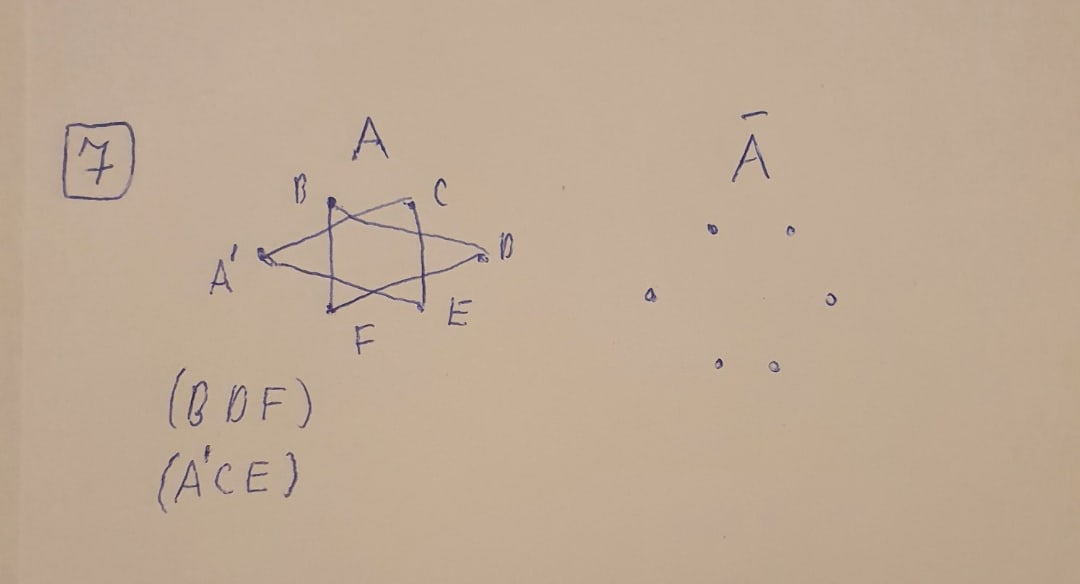
\includegraphics[scale=0.4]{5.jpg}

\includegraphics[scale=0.2]{25531.eps}
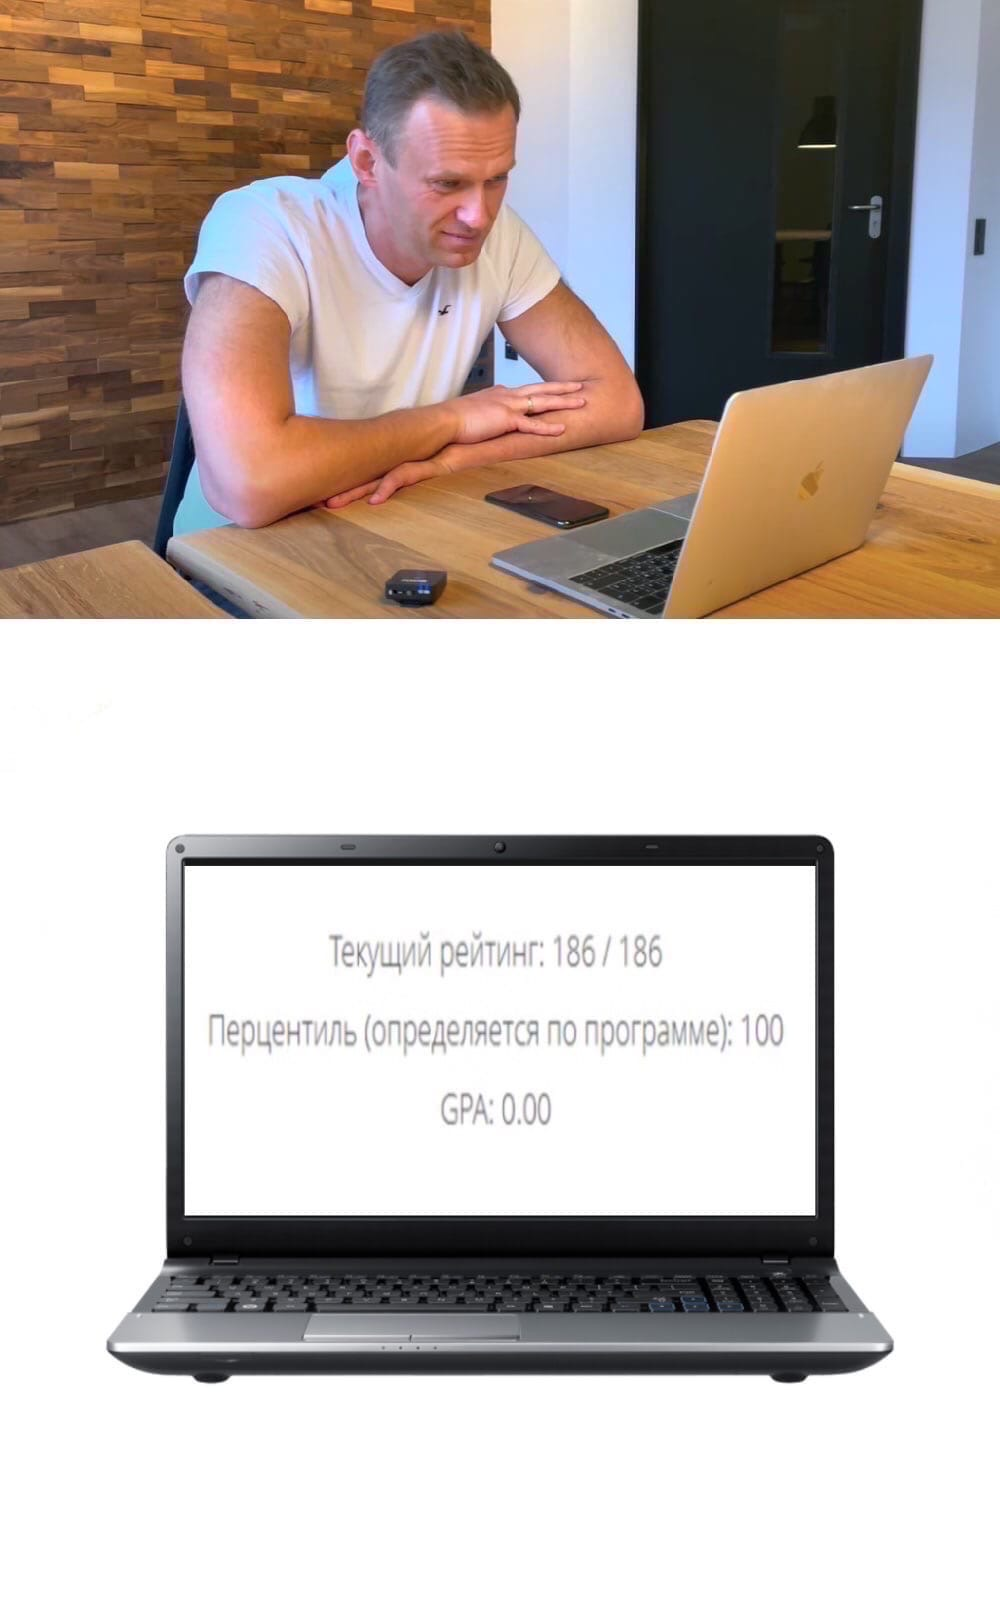
\includegraphics[scale=0.4]{4jpg.jpg}
\end{center}
\section*{Номер 8} 
\subsection*{а)}
\[
f (x) = \frac{3x-7}{(x^2-1)^2}
\]
\[
f'(x) = \frac{3(x^2-1)^2 - 2(x^2-1) \cdot 2x(3x-7)}{(x^2-1)^4} =
\]
\[
= \frac{(x^2-1)\left[3(x^2-1) - 4x(3x-7)\right]}{(x^2-1)^4} = \frac{-9x^2+28x - 3}{(x^2-1)^3}
\]
Найдем точки, в которых производная обращается в ноль:
\[
-9x^2 + 28x -3 = 0
\]
\[
x_1 = \frac{1}{9}, x_2 = 3
\]
Найдем точки разрыва функции:
\[
x_3 = -1, x_4 = 1
\]
Итого:
\begin{center}
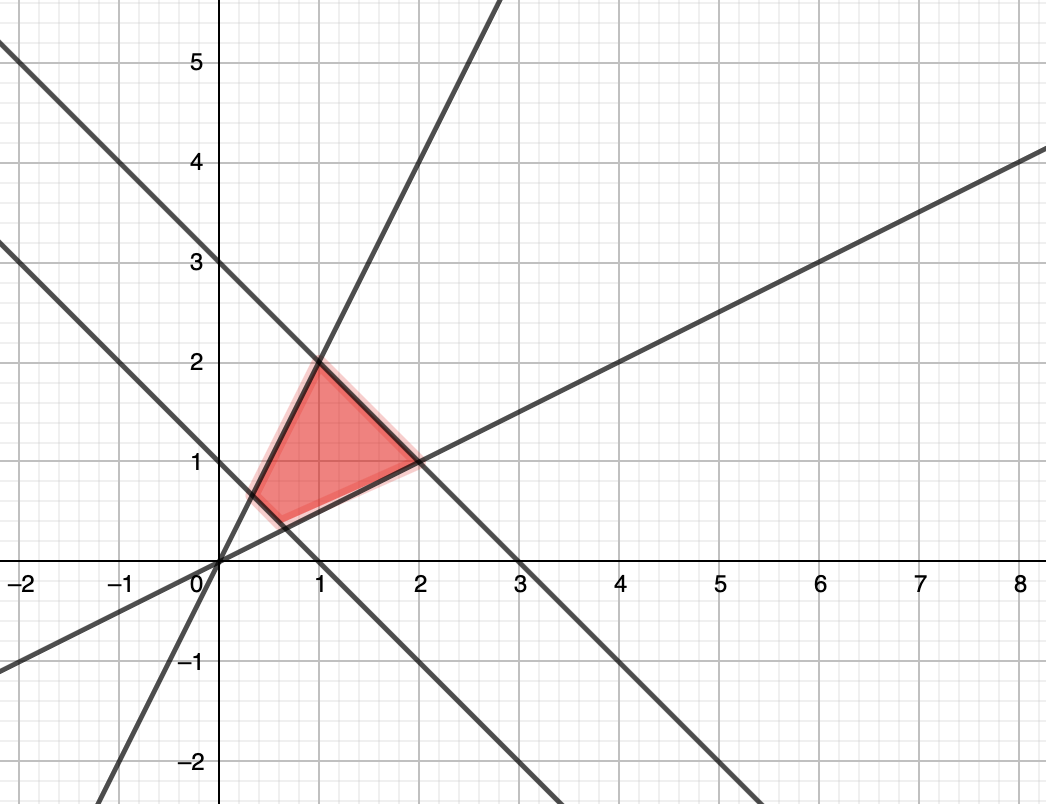
\includegraphics[scale=0.4]{1.png}
\end{center}
А значит:
\begin{itemize}
\item Функция убывает на:
\[
(-\infty; -1)
\]
\[
\left( \frac{1}{9}; 1 \right)
\]
\[
(3; \infty)
\]
\item Функция возрастает на:
\[
\left( -1;\frac{1}{9} \right)
\]
\[
(1;3)
\]
\item Точки максимума:
\[
\frac{1}{9}; 3
\]
\item Точки минимума:
\[
-1; 1
\]
\end{itemize}


\subsection*{b)}
\[
f(x) = \frac{(\text{ln }x)^2}{\sqrt{x}}
\]
\[
f'(x) = 
\frac{\frac{1}{x} \cdot 2 \text{ln } x \cdot \sqrt{x} - \frac{(\text{ln } x)^2}{2\sqrt{x}}}{x} = \frac{\text{ln } x \cdot (4 - \text{ln } x)}{2x \cdot \sqrt{x}}
\]
Найдем точки, в которых производная обращается в ноль:
\[
x_1 = 1; x_2 = e^4
\]
Найдем точки разрыва функции:
\[
x_3 = 0
\]
Итого:
\begin{center}

\includegraphics[scale=0.4]{2.png}
\end{center}
А значит:
\begin{itemize}
\item Функция убывает на:
\[
\left( 0; 1\right)
\]
\[
\left( e^4; \infty \right)
\]

\item Функция возрастает на:
\[
\left( 1; e^4 \right)
\]

\item Точки максимума:
\[
e^4
\]
\item Точки минимума:
\[
1
\]
\end{itemize}
\subsection*{с)}
\[
f(x) = \frac{2x}{1+x^2}
\]
\[
f'(x) = \frac{2(1+x^2) - 4x^2}{(1+x^2)^2} 
=
\frac{2-2x^2}{(1+x^2)^2}
\]
Найдем точки, в которых производная обращается в ноль:
\[
2 - 2x^2 = 0
\]
\[
x_1 = -1, x_2 = 1
\]
\\\\
Итого:
\begin{center}
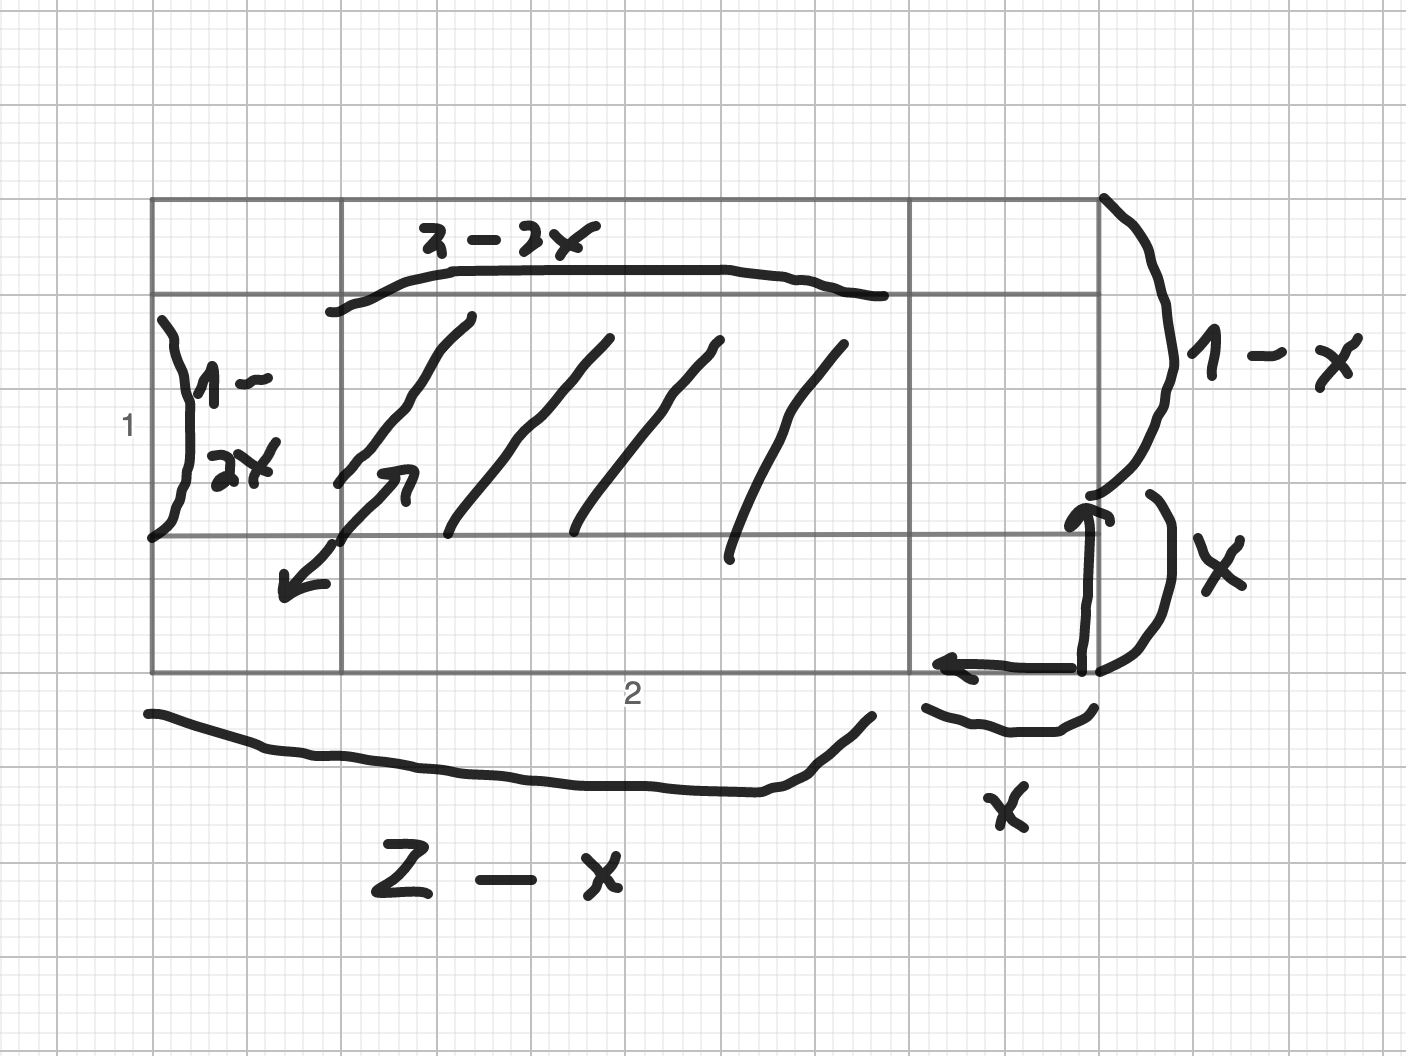
\includegraphics[scale=0.3]{3.png}
\end{center}
А значит:
\begin{itemize}
\item Функция убывает на:
\[
(-\infty; -1)
\]
\[
(1; \infty)
\]
\item Функция возрастает на:
\[
\left( -1 ; 1 \right)
\]

\item Точки максимума:
\[
1
\]
\item Точки минимума:
\[
-1
\]
\end{itemize}
\section*{Номер 9}
\subsection*{a)}
\[
1 + \frac{x}{2} - \frac{x^2}{8} \leq \sqrt{1+x} \leq 1 + \frac{x}{2}, \; x > 0
\]
\begin{enumerate}
\item
\[
f = 1 + \frac{x}{2} - \frac{x^2}{8} \leq g = \sqrt{1+x}
\]
\[
f(0) = g(0) = 1;
\]
\[
f' = \frac{1}{2} - \frac{x}{4}, \; g' = \frac{1}{2\sqrt{1+x}}
\]
\[
f'(0) = g'(0) = \frac{1}{2}
\]
\[
f'' = -\frac{1}{4}
\]
\[
g'' = -\frac{1}{4} \cdot \frac{1}{(1+x)\sqrt{1+x}}
\]
Т.к $x \geq 0$, то:
\[
g'' \geq f'' \rightarrow g' \geq f' \rightarrow g \geq f
\]
\item
\[
f(x) = \sqrt{1+x} \leq g(x) =1 + \frac{x}{2}
\]
\[
f(0) = g(0) = 1
\]
\[
f' = \frac{1}{2\sqrt{1+x}}, \; g' = \frac{1}{2}
\]
\[
g' \geq f' \rightarrow g \geq f
\]
\end{enumerate}
\begin{center}
\textbf{Ч.Т.Д}
\end{center}
\subsection*{b)}
\[
e^{x-1} + \text{ln } x - 2x + 1 \geq 0, \; x \geq 1
\]
\[
f(x)= e^{x-1} +1 \geq g(x) = 2x - \text{ln } x
\]
\[
f(1) = g(1) = 2
\]
\[
f' = e^{x-1},\;  g' = 2 - \frac{1}{x}
\]
\[
f'(1) = g'(1) = 1
\]
\[
f'' = e^{x-1}, g'' = \frac{1}{x^2}
\]
\[
f''(1) = g''(1) = 1
\]
\[
f''' = e^{x-1}, g''' = -\frac{2}{x^3}
\]
Т.к $x \geq 1$, то $e^{x-1} \geq -\frac{2}{x^3}$, а значит:
\[
f''' \geq g''' \rightarrow f'' \geq g'' \rightarrow f' \geq g' \rightarrow f \geq g
\]
\begin{center}
\textbf{Ч.Т.Д}
\end{center}
\subsection*{c)}
\[
\frac{b-a}{b} < \text{ln } \frac{b}{a} < \frac{b-a}{a}, \; 0 < a < b
\]
Т.к a > 0, то сделаем замену $\frac{b}{a} = t$, тогда:
\[
1 - \frac{1}{t} < \text{ln } t < t - 1
\]
\begin{enumerate}
\item
\[
f(t) = 1 - \frac{1}{t} < g(t) = \text{ln } t
\]
\[
f(1) = g(1) = 0
\]
\[
f' = \frac{1}{t^2}, \; g' = \frac{1}{t}
\]
Поскольку $t = \frac{b}{a}$ и $ b > a  > 0$, то $t > 1$ и $t^2 > t$, а значит:
\[
g' > f' \rightarrow g > f
\]
\item
\[
f(t) = \text{ln } t < g(t) =  t - 1
\]
\[
f(1) = g(1) = 0
\]
\[
f' = \frac{1}{t}, \; g' = 1
\]
Поскольку $ b > a$, то $t \neq 1$, а значит $\frac{1}{t} < 1$:
\[
g' > f' \rightarrow g > f
\]
\begin{center}
\textbf{Ч.Т.Д}
\end{center}
\end{enumerate}
\end{document}